\subsection{L-diversité}
%ajout d'exeple

La l-diversité est une technique d’agrégation qui étend la k-anonymisation. En effet, il est toujours possible de déduire les informations sensibles si les k individus d’une classe d’équivalence possèdent tous la même information sensible Figure \ref{fig:Données 3-anonymes mais pas l-diverses}

La l-diversité ajoute une contrainte selon laquelle les k-enregistrements d’une classe d’équivalence doivent avoir au minimum l valeurs distinctes comme dans la figure \ref{fig:Données 3-anonymes et 3-diverses}

%ajout d'exemple

Dans l’exemple \ref{fig:Données 3-anonymes mais pas l-diverses}, si l’on sait qu’une personne cultive une grande culture (blé, mais, orge) on déduit quel type de pesticides elle utilise, dans notre cas, les fongicides (\textbf{\textbf{homogeneity Attack}}).  Comme citer en haut, l’inférence est la grande faiblesse du k-anonymat.La l-diversité vient y remédier en y ajout une contrainte Figure \ref{fig:Données 3-anonymes et 3-diverses}. 

Ainsi donc on n’est plus en mesure de deviner le type de pesticides utilisé en fonction du type de culture.  

Cependant, avec un attaque d’inférence probabiliste, on peut par exemple déduire avec une certaine probabilité assez élevée, le type de pesticide utilisé. En effet, si la personne malveillante sait qu’Alan, qui est la seule personne à avoir une parcelle de 38ha, alors, il lui est possible de deviner, avec une probabilité de 1/3, le type de pesticide qu’Alan utilise (\textit{\textbf{Background Knowledge Attack}}). 
\begin{figure}[!h]
    \centering
      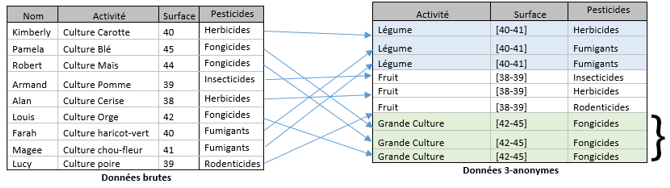
\includegraphics[width=1\textwidth]{images/anonymisation/l_divers_image1.png}
    \caption{ Données 3-anonymes mais pas l-diverses}
     \label{fig:Données 3-anonymes mais pas l-diverses}
   
\end{figure}


\begin{figure}[!h]
    \centering
      
   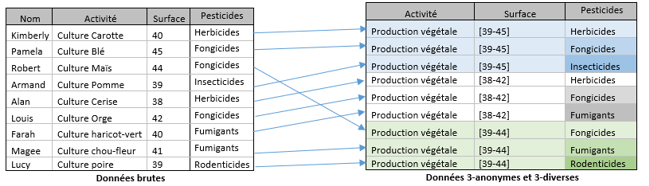
\includegraphics[width=1\textwidth]{images/anonymisation/l_divers_image2.png}
    \caption{Données 3-anonymes et 3-diverses }
     \label{fig:Données 3-anonymes et 3-diverses}
\end{figure}

\paragraph{Evaludation de L-diversité : }
\begin{itemize}
    \item \textbf{Individualisation:} la l-diversité empêche que les enregistrements relatifs à un individu soient isolés dans la base de données 

   \item \textbf{Corrélation:} la l-diversité n’apporte pas d’amélioration par rapport au k-anonymat.  

   \item \textbf{Inférence:} bien qu’il ne soit plus possible de faire des attaques par inférence, il reste cependant possible de mener des attaques par inférence probabiliste. 
\end{itemize}


